\chapter{绪论}
\section{星系形态学}
星系形态学作为现代天文学和天体物理学的核心研究领域之一,为理解宇宙中最复杂的恒星系统~——~星系的形成与演化过程提供了重要的观测窗口\cite{Kormendy2004,Sandage2005,Mo2010,Conselice2014}。自Edwin Hubble在1926年首次建立系统性的星系分类体系\cite{Hubble1926}以来,并经由de Vaucouleurs等人的进一步发展和完善,星系形态学研究已经从最初的经验性分类发展成为连接观测天文学与理论天体物理学的重要桥梁。


\begin{figure}[htbp]
\centering
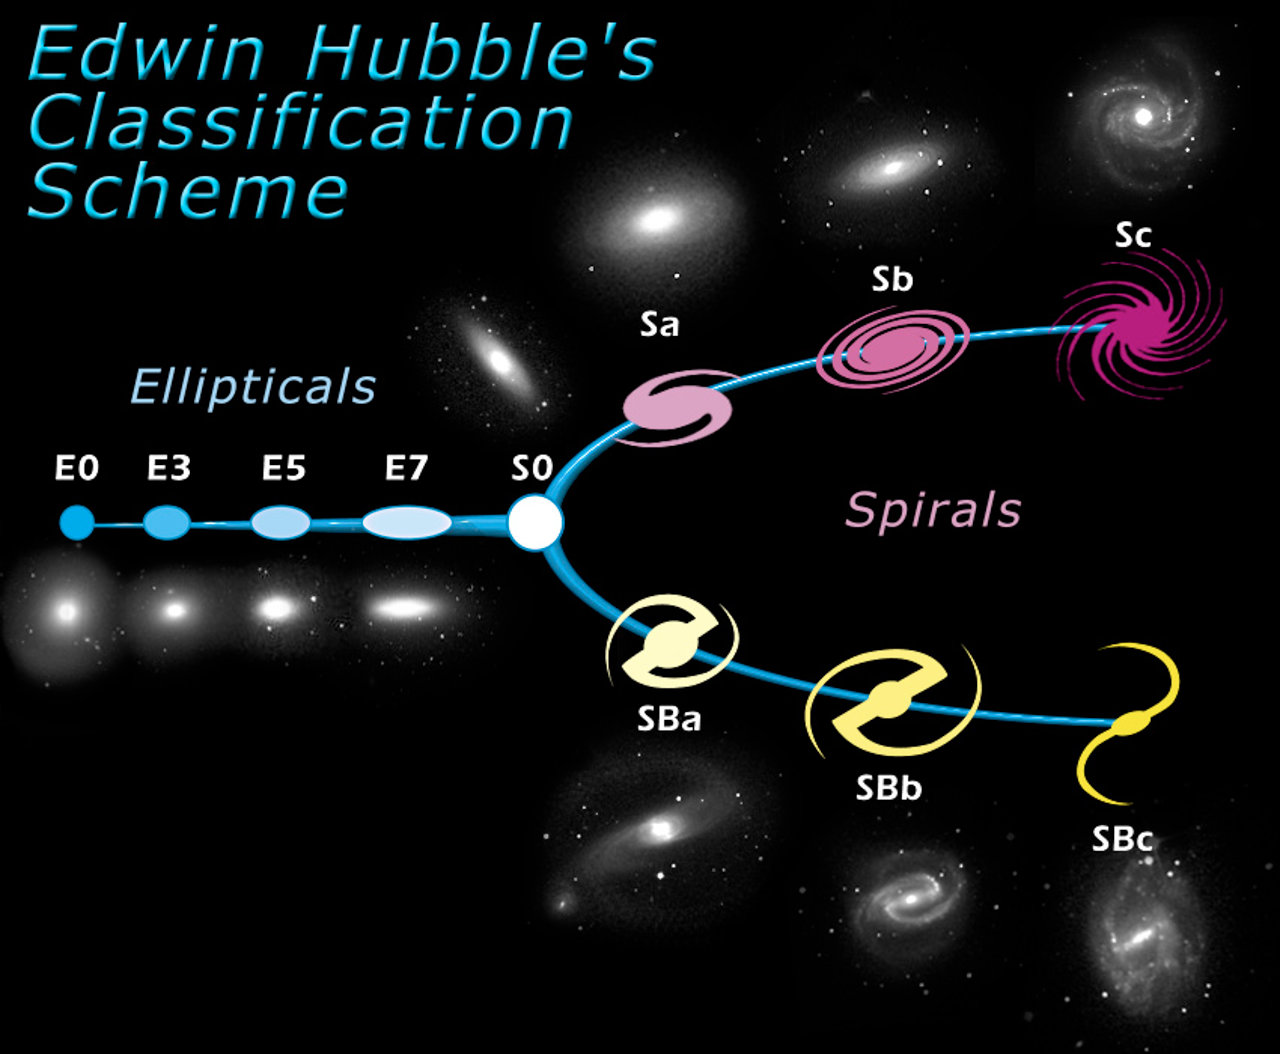
\includegraphics[width=0.45\textwidth]{Hubble_Sequence.jpg}
\caption{: \emph{Hubble Sequence示意图。左侧为椭圆星系序列(E0-E7),按照扁率递增排列,从近似球形(E0)到高度扁平(E7);中央为透镜状星系(S0),具有明显的核球和盘结构但缺乏螺旋臂特征;右侧分别为正常螺旋星系(Sa-Sc)和棒旋星系(SBa-SBc)序列,展现了从紧密缠绕的旋臂结构到疏松开放的旋臂形态的连续变化。图片来源:NASA\&ESA 。}}
\label{fig:hubble_sequence}
\end{figure}

所有参数的具体分布见表\ref{tab:simulation_parameters}:

\begin{table}[htbp]
\centering
\caption{模拟星系参数设置}
\label{tab:simulation_parameters}
\begin{tabular}{lc}
\hline
\hline
\textbf{参数} & \textbf{取值范围} \\
\hline
总星等 ($m_{\text{total}}$) & 20-28 AB mag \\
B/T比值 & 10\%-90\% \\
核球有效半径 ($R_{\text{bulge}}$) & 0\farcs05-0\farcs2 \\
盘有效半径 ($R_{\text{disc}}$) & 1.5-3.0 × $R_{\text{bulge}}$ \\
核球轴比 ($q_{\text{bulge}}$) & 0.8-0.9 \\
盘轴比 ($q_{\text{disc}}$) & 0.4-0.7 \\
核球Sérsic指数 ($n_{\text{bulge}}$) & 4.0 (固定) \\
盘Sérsic指数 ($n_{\text{disc}}$) & 1.0 (固定) \\
\hline
\hline
\end{tabular}
\end{table}

Sérsic轮廓作为描述星系表面亮度分布的核心数学工具,其一般形式可表示为:
\begin{equation}
I(R) = I_e \exp\left\{-k\left[\left(\frac{R}{R_{\text{eff}}}\right)^{1/n} - 1\right]\right\}
\end{equation}
\subsection{现代宇宙学框架下的星系形态演化}



